\begin{figure*}
 \centerline{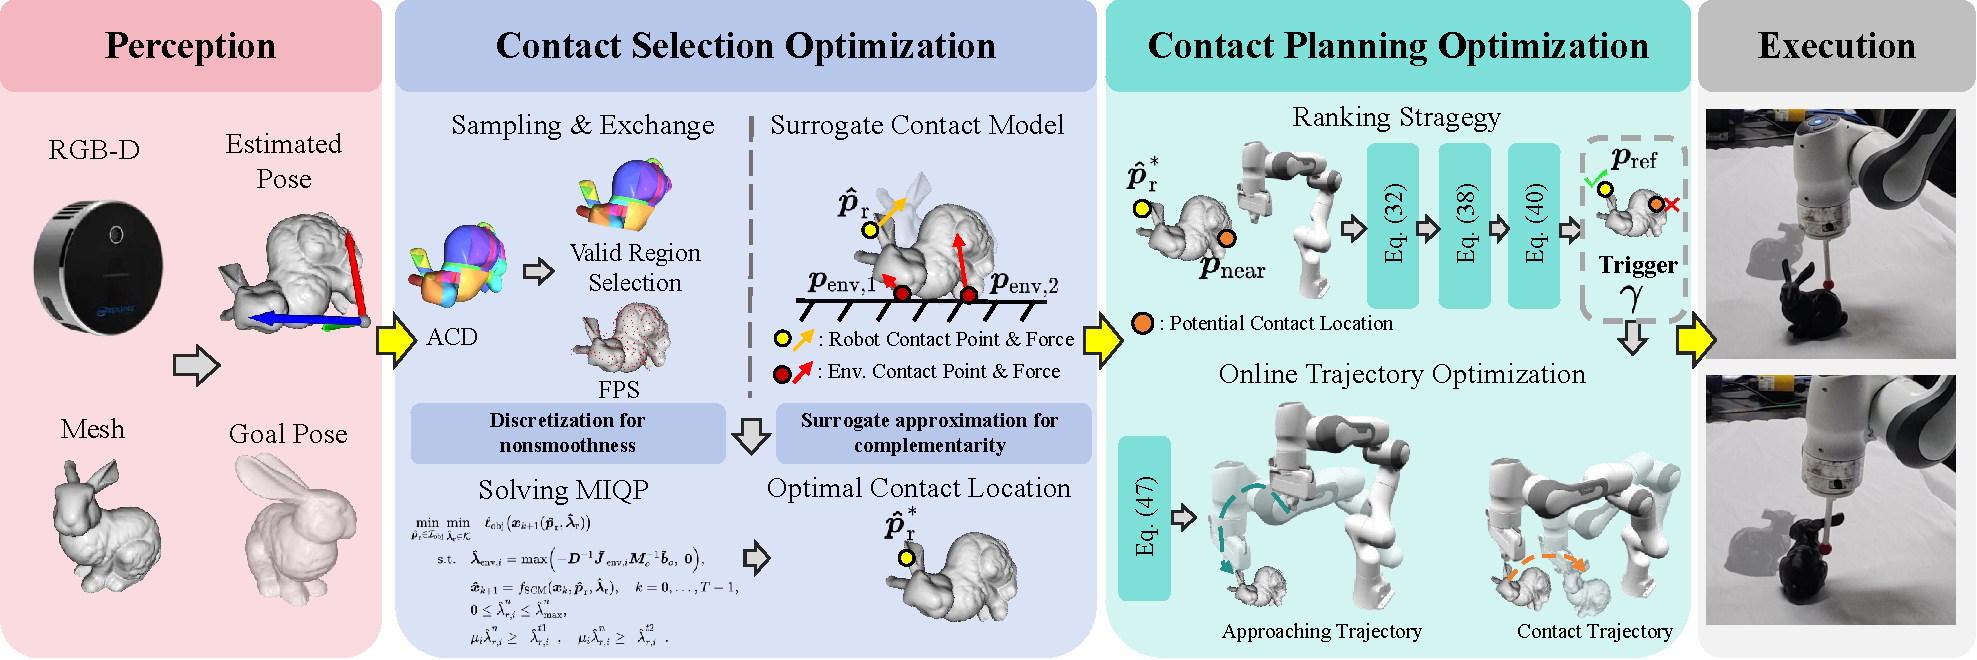
\includegraphics[width=\textwidth]{figures/framework.pdf}}
\caption{Framework structure of SCSP. SCSP consists of Contact Selection Optimization (CSO) and Contact Planning Optimization (CPO). CSO discretizes nonsmooth geometry through the Sampling \& Exchange method and introduces a surrogate contact model for efficient approximation of contact dynamics. CSO online computes the \rev{optimal contact location among candidate contact set} $\boldsymbol{\hat{p}}_{\text{r}}^*$ as contact prior. The ranking strategy in CPO further evaluates whether the nearest point $\boldsymbol{p}_{\text{near}}$ can serve as a feasible suboptimal substitute for $\boldsymbol{\hat{p}}_{\text{r}}^*$ as the reference contact location, after which trajectory optimization is solved online to generate the approach and contact trajectories.}
\label{fig:framework}
\end{figure*}

\section{Contact Selection Optimization}
\label{sec:cso}

In this section, we present the detailed design of CSO.
We begin by analyzing the key challenges of integrating contact selection into CIMPC, which limit the diversity of existing methods.
\textcolor{blue}{
We then formulate the contact selection problem and discuss the main difficulties in solving it.
}
Finally, we present the detailed design of our CSO module for online contact selection.


\subsection{Why Contact Selection is necessary?} 

\textcolor{red}{Contact selection refers to choosing object contact locations $\left \{ \boldsymbol{p}_{\mathcal{O}, i} \right \} \subset \partial \mathcal{O}$ that can generate task-beneficial wrenches for changing the object pose. According to \eqref{equ.quasi_dyn_1} and \eqref{equ.quasi_dyn_2}, the object wrench is jointly determined by the contact Jacobian, which depends on the contact location and its local geometry, and the contact impulse $\boldsymbol{\beta}_i$ (or, equivalently, the contact force $\boldsymbol{\lambda}_i$). For some contact locations, no force within the corresponding friction cone can produce a wrench that improves the object pose; contact switching is therefore necessary.}

\textcolor{red}{CIMPC models robot--object interaction (ROI) with contact dynamics whose informative gradients are confined to the low-dimensional contact manifold $\mathcal{S}_{\text{contact}}$ embedded in the full state space $\mathcal{S}$. The contact-free manifold $\mathcal{S}_{\text{free}}$ provides no effective contact-induced gradient, making autonomous contact selection difficult and requiring attractive costs or reference trajectories to induce contact. Although CIMPC can choose between contact and non-contact modes, its short receding horizon may not reveal, within the fixed horizon, the benefit of reaching a distant contact location.}

Rather than integrating contact selection into the CIMPC formulation, we study how to formulate contact selection as a separate optimization problem. As illustrated in Fig. \ref{fig:framework}, we first simplify the problem by ignoring the planning of the robot contact locations $\left \{ \boldsymbol{p}_{\mathcal{R}, i} \right \}$ and thereby obtain the following object-centric optimization problem:
\begin{equation}
    \begin{aligned}
        \min_{\boldsymbol{p}_{\text{r}} \in \partial \mathcal{O}, \boldsymbol{\lambda} \in \mathcal{K}} & 
        \ell_{\text{cso}}(\boldsymbol{x}_{\textcolor{red}{T}}) \\
        \text{s.t.} \quad 
        & \boldsymbol{x}_{k+1} = f(\boldsymbol{x}_k, \boldsymbol{p}_{\text{r}}, \boldsymbol{\lambda}),
        \quad k = 0, \dots, T-1.
    \end{aligned}\label{scsp}
\end{equation}
where $\mathcal{K}$ is the set of feasible contact forces and $\ell_{\text{cso}}(\cdot)$ is the objective of contact selection. $\boldsymbol{p}_{\text{r}} \in \mathbb{R}^{3 \times n_{\text{r}}}$ represents the locations where the robot applies contacts to the object, with $n_{\text{r}}$ denotes the number of robot contacts. \eqref{scsp} addresses the gradient sparsity issue arising from hybrid planning in the original contact-rich manipulation problem by defining CSO to solve for \rev{low-cost sampled contact locations} and contact forces on $\mathcal{S}_{\text{contact}}$. The neglected process of the robot approaching $\mathcal{S}_{\text{contact}}$ from its current state is the primary source of the gradient sparsity. Note that \eqref{scsp} is hard to solve due to the coupling of contact location $\boldsymbol{p}_{\text{r}}$ and the contact force $\boldsymbol{\lambda}=\left [ \boldsymbol{\lambda}_{\text{env}}, \boldsymbol{\lambda}_{\text{r}} \right ]$. Therefore, we adopt a commonly used simplification for handling nonconvex optimization problems to reformulate (\ref{scsp}) as subproblems:
\begin{equation}
    \min_{\boldsymbol{p}_{\text{r}} \in \partial \mathcal{O}}
    \quad V(\boldsymbol{p}_{\text{r}})\label{equ:outer_loop},
\end{equation}
in which:
\begin{equation}
\begin{aligned}
V(\boldsymbol{p}_{\text{r}})
:= \min_{\boldsymbol{\lambda}_{\text{r}} \in \mathcal{K}} \quad &
\ell_{\text{cso}}(\boldsymbol{x}_{\textcolor{red}{T}}) \\
\text{s.t.} \quad
& \boldsymbol{x}_{k+1}
= f(\boldsymbol{x}_k, \boldsymbol{p}_{\text{r}}, \boldsymbol{\lambda}_{\text{r}}, \boldsymbol{\lambda}_{\text{env}}),
\quad k = 0, \dots, T-1.
\end{aligned}\label{equ:inner_loop}
\end{equation}
The physical interpretation of \eqref{equ:outer_loop} and \eqref{equ:inner_loop} is that a contact location is regarded as optimal if applying the best possible combination of contact force $\boldsymbol{\lambda}^*$ yields the minimum motion cost of the object. Despite the simplifications, \eqref{equ:outer_loop} remains a complex problem with nonsmooth constraints $\boldsymbol{p}_{\text{r}} \in \partial \mathcal{O}$ that depend on the object geometry. Meanwhile, \eqref{equ:inner_loop} is a complementary problem with coupled environment forces $\boldsymbol{\lambda}_{\text{env}}$ and robot contact forces $\boldsymbol{\lambda}_{\text{r}}$. The nonconvexity makes online CSO intractable. We next present the solutions to further simplify both \eqref{equ:outer_loop} and \eqref{equ:inner_loop} to improve computational efficiency. 



\subsection{Sampling and Exchange Method}\label{sec:sampling&exchange}
The nonsmoothness on the object geometry leads to discontinuities in the gradient of \eqref{equ:outer_loop}. The inherently nonsmooth nature of the problem motivates us to adopt a sampling-based method. To simplify \eqref{equ:outer_loop}, we uniformly sample a set of candidate contact point set $\mathcal{I}_{\text{obj}} = \{\boldsymbol{p}_i\}_{i=1}^{n_s}$ on the object surface $\partial \mathcal{O}$, thus reformulate \eqref{equ:outer_loop} as:
\begin{equation}
    \min_{\boldsymbol{p}_{\text{r}} \in \mathcal{I}_{\text{obj}}}
    \quad V(\boldsymbol{p}_{\text{r}}),\label{equ:simplify_outer_loop}
\end{equation}
When the sampling is sufficiently uniform, \eqref{equ:simplify_outer_loop} provides a good approximation to \eqref{equ:outer_loop} and is not affected by discontinuous gradients caused by the geometry. To obtain a high quality candidate set, $\mathcal{I}_{\text{obj}}$ should satisfy the following conditions:
\begin{itemize}
    \item \textbf{Physical reachability}, which requires that candidate contact locations be reachable by the robot, i.e., within the robot workspace and not occluded.
    \item \textbf{Contact stability}, which requires avoiding regions with high curvature where stable contact is difficult to apply.
    \item \textbf{Uniform distribution}, which means the sampled points are representative of approximating the original geometry.
\end{itemize}
These conditions require the sampling method to maintain uniform coverage while prioritizing manipulability over local geometric details. To address this, we propose an efficient sampling strategy as shown in Algorithm \ref{algorithm:sampling}. We first perform approximate convex decomposition (ACD) \cite{lien2007approximate} to obtain a convex approximation $\mathcal{F}$ of the original geometry $\mathcal{O}$. ACD decomposes the object into convex polygons, mitigating interference caused by local geometric details and reducing computational cost. Moreover, these polygons are typically larger and flatter, which implies greater contact stability and improved reachability.

Then we perform Farthest-Point Sampling (FPS) on the convex approximation to uniformly sample points on the polygons. Starting from an arbitrary point as a sample, the algorithm iteratively selects the points that maximize the minimal Euclidean distance to all previously chosen samples:
\begin{equation}
p'_{k+1} = \arg\max_{p_i \in \mathcal{F}} \min_{p'_j \in \mathcal{I}_{k}} \|\boldsymbol{p}_i - \boldsymbol{p}'_j\|^2, \label{equ:FPS}
\end{equation}
where $\mathcal{I}_{k}$ is the set of already selected samples. The sampling process is performed offline. Solving \eqref{equ:FPS} yields a uniformly distributed set of points $\mathcal{I}_{\text{obj}}$. For each sampled point $p'_j \in \mathcal{I}_{k}$, we also construct its local coordinate frame to obtain the tangential and normal vectors as local contact information. The local orthonormal frame is constructed as $(\boldsymbol{n}_i, \boldsymbol{t}_{1,i}, \boldsymbol{t}_{2,i})$ in which the normal vector $\boldsymbol{n}_i$ is obtained from the mesh or point-cloud normal estimate, and two orthogonal tangent directions are computed as:
\begin{equation}
\boldsymbol{t}_{1,i} = 
\frac{\boldsymbol{a} - (\boldsymbol{a} \cdot \boldsymbol{n}_i)\boldsymbol{n}_i}
{\|\boldsymbol{a} - (\boldsymbol{a} \cdot \boldsymbol{n}_i)\boldsymbol{n}_i\|}, \ 
\boldsymbol{t}_{2,i} = \boldsymbol{n}_i \times \boldsymbol{t}_{1,i},
\end{equation}
where $\boldsymbol{a}$ is an arbitrary fixed axis. \textcolor{red}{When the reference axis $a$ is nearly parallel to the surface normal $n_i$, we select another coordinate axis as the reference axis to avoid numerical singularity.} We use this local geometric information to compute the Jacobian required for contact force optimization. Furthermore, a KD-tree $\mathcal{T}=\left \{ (\boldsymbol{p}_i,\boldsymbol{n}_i, \boldsymbol{t}_{1,i}, \boldsymbol{t}_{2,i}) \right \}^{n_s}_{i=1} $ is constructed over the set $\mathcal{I}_{\text{obj}}$ to enable efficient nearest-neighbor queries.

An online Valid Region Selection procedure is further applied to identify feasible and task-relevant surface regions, filtering out unreachable or low-quality points such as occluded regions, regions outside the robot workspace, and \rev{regions that violate task-specific semantic masks (for example, handles or forbidden surfaces).} The valid region is maintained by applying a mask to $\mathcal{F}$ to obtain $\mathcal{F}_{\text{v}}$, and then selecting points on $\mathcal{F}_{\text{v}}$ to obtain $\mathcal{I}_{\text{avail}}$. To better illustrate the process, consider the toy example shown in Fig. \ref{fig:FPS}. First, following the procedure illustrated in Fig. \ref{fig:FPS}(a), we iteratively apply \eqref{equ:FPS} to obtain a set of uniformly distributed sampling points over the processed object mesh. We then partition the surface online into a set of valid regions and masked regions, and select the points that lie within the valid regions to form the candidate set $\mathcal{I}_{\text{avail}}$, as shown in Fig. \ref{fig:FPS}(b).

\begin{figure}[!t]
 \centerline{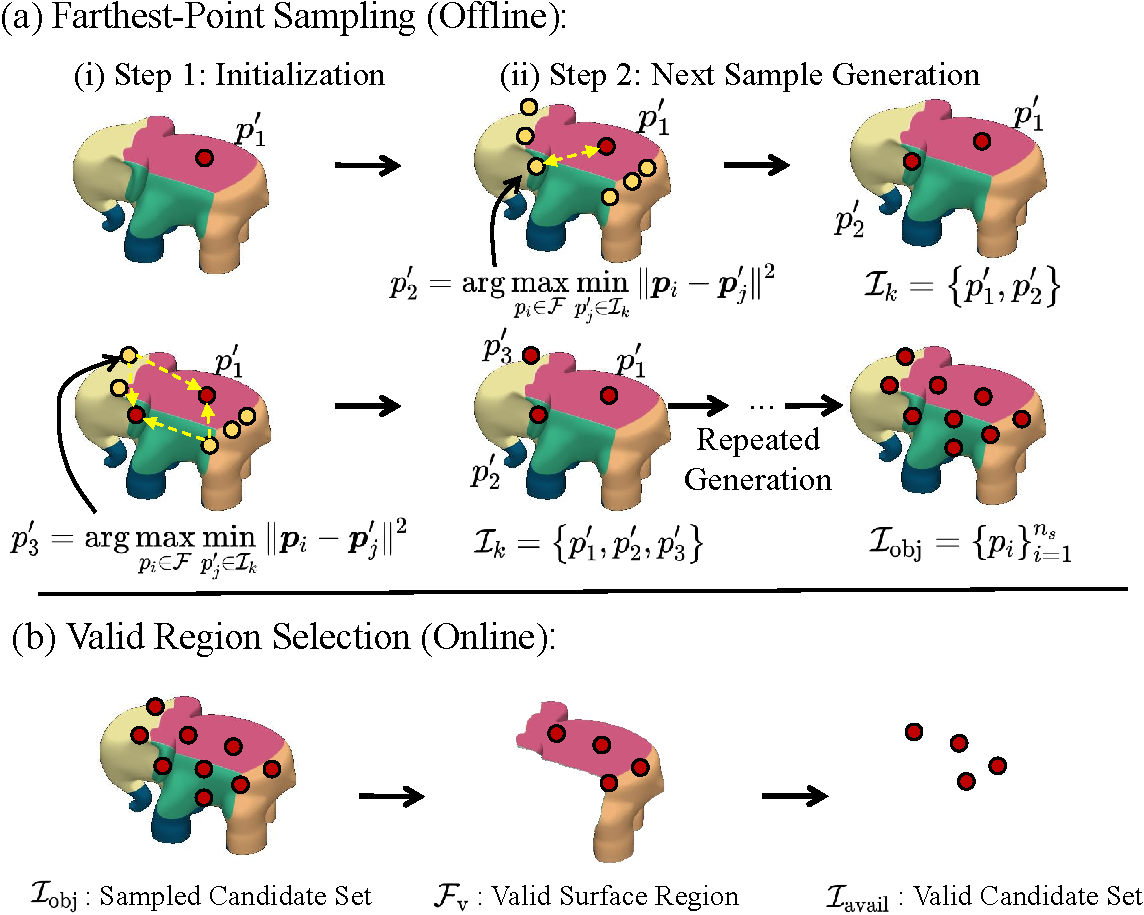
\includegraphics[width=\columnwidth]{figures/sampling_strategy.pdf}}
\caption{The sampling strategy in CSO. The candidate point set is sampled sequentially through: (a) Farthest-Point Sampling to uniformly sample points on the object, and (b) Valid Region Selection to select valid points for contact.}
\label{fig:FPS}
\end{figure}

\begin{algorithm}[t]
\caption{Sampling and Exchange Method}
\label{algorithm:sampling}
\begin{algorithmic}[1]
\Require Object geometry $\mathcal{O}$, sample count $K$, fixed axis $\boldsymbol{a}$
\Ensure $\mathcal{T}= \left \{ (\boldsymbol{p}_i,\boldsymbol{n}_i, \boldsymbol{t}_{1,i}, \boldsymbol{t}_{2,i}) \right \}^{n_s}_{i=1}$ and $\mathcal{I}_{\text{avail}}$.

\State $\mathcal{F} \gets \text{ACD}(\mathcal{O})$ \Comment{Convex approximation}
\State Initialize $\mathcal{I}_{k} \gets \{p'_1\}$ with an arbitrary seed in $\mathcal{F}$
\For{$k=1$ to $K-1$}
    \State $p'_{k+1} \gets \arg\max_{p'_i\in \mathcal{F}} \min_{p_j\in \mathcal{I}_{k}} \|\boldsymbol{p}'_i-\boldsymbol{p}'_j\|^2$
    \State $\mathcal{I}_{\text{obj}} \gets \mathcal{I}_{k} \cup \{p'_{k+1}\}$ \Comment{Obtain candidate set $\mathcal{I}_{\text{obj}}$}
\EndFor
\State $\mathcal{F}_{\text{v}} \gets \text{getValidRegion}(\mathcal{F})$ \Comment{Task-specific segment}
\ForAll{$p_i \in \mathcal{I}_{\text{obj}}$}
    \If{$p_i \notin \mathcal{F}_{\text{v}}$}
        \State Remove $p_i$ from $\mathcal{I}_{\text{obj}}$ \Comment{Valid region selection}
        \State \textbf{continue}
    \EndIf \Comment{Obtain $\mathcal{I}_{\text{avail}}$}
    \State Estimate normal $\boldsymbol{n}_i$ from $\mathcal{F}$ at $p_i$
    \State $\boldsymbol{t}_{1,i} \gets \dfrac{\boldsymbol{a}-(\boldsymbol{a}\cdot\boldsymbol{n}_i)\boldsymbol{n}_i}{\|\boldsymbol{a}-(\boldsymbol{a}\cdot\boldsymbol{n}_i)\boldsymbol{n}_i\|}$, \ $\boldsymbol{t}_{2,i} \gets \boldsymbol{n}_i \times \boldsymbol{t}_{1,i}$
\EndFor
\State \Return $\mathcal{T}=\left \{ (\boldsymbol{p}_i,\boldsymbol{n}_i, \boldsymbol{t}_{1,i}, \boldsymbol{t}_{2,i}) \right \}^{n_s}_{i=1}$
\end{algorithmic}
\end{algorithm}

\subsection{Surrogate Contact Model}

The sampling strategy transforms the original optimization into a discrete–continuous optimization problem. We further simplify \eqref{equ:inner_loop} to improve efficiency. Most existing contact models are computationally expensive for scenarios that require repeatedly solving \eqref{equ:inner_loop}. Moreover, the complementarity in contact dynamics and the coupling between $\boldsymbol{\lambda}_{\text{env}}$ and $\boldsymbol{\lambda}_{\text{r}}$  make the optimization difficult to converge, leading to physically inconsistent results. To address this issue and enable online contact selection, we present a surrogate contact model (SCM) as a local approximation of the original contact dynamics. The procedure of SCM is illustrated in Fig. \ref{fig:stick1}. The approximation relies on the following assumptions of the object-environment contact:

\begin{assumption}[Fixed Contact Set]
 The object--environment contact location remains unchanged in each SCM rollout, i.e., no new contacts are created and existing contacts remain.\label{assumption:mode}
\end{assumption}

\begin{assumption}[Multi-Contact Decoupling]
 The contact between the object and the environment can be approximated by independent spring–damper systems, neglecting higher-order dynamic couplings between different contact locations. \label{assumption:decoupling}
\end{assumption}

We reformulate the original contact dynamics in (\ref{equ.quasi_dyn_1}) as:
\begin{equation}
    \epsilon\boldsymbol{M}_o\boldsymbol{v}_o = 
    h(\boldsymbol{\tau}_o+\sum\nolimits_{i=1}^{n_{\text{r}}}{\boldsymbol{J}}_{\text{r},i}^{\top}\boldsymbol{\lambda}_{\text{r},i} + \sum\nolimits_{j=1}^{n_{\text{env}}}{\boldsymbol{J}}_{\text{env},j}^{\top}\boldsymbol{\lambda}_{\text{env},j}),
    \label{eq:simplified}
\end{equation}
and we denote $\boldsymbol{\tilde{b}}_o = h(\boldsymbol{\tau}_o+\sum\nolimits_{i=1}^{n_{\text{r}}}{\boldsymbol{J}}_{\text{r},i}^{\top}\boldsymbol{\lambda}_{\text{r},i})$. Similar to (\ref{equ.dual_prob_relax}), the physically consistent environment contact force can be obtained by solving the following dual problem:
\begin{multline}
\max_{\boldsymbol{\lambda}_{\text{env}}\geq \boldsymbol{0}}\quad  
    -\frac{1}{2} \boldsymbol{\lambda}_{\text{env}}^\top 
    \left(
    \boldsymbol{\tilde{J}}_{\text{env}} \boldsymbol{M}_o^{-1} \boldsymbol{\tilde{J}}_{\text{env}}^\top
    +\boldsymbol{R}
    \right) 
    \boldsymbol{\lambda}_{\text{env}} \\
    -
    (\boldsymbol{\tilde{J}}_{\text{env}} \boldsymbol{M}_o^{-1}\boldsymbol{\tilde{b}}_o+\boldsymbol{\tilde{\phi}})^\top
    \boldsymbol{\lambda}_{\text{env}}
    -\frac{1}{2} 
    \boldsymbol{\tilde{b}}_o^\top
    \boldsymbol{M}_o^{-1}
    \boldsymbol{\tilde{b}}_o,
    \label{eq:dual_problem}
\end{multline}
and the solution satisfies the complementarity condition
\begin{equation}
\boldsymbol{0}\leq \boldsymbol{\lambda}_{\text{env}} \perp
\boldsymbol{W}_{\text{env}}
\boldsymbol{\lambda}_{\text{env}}
+\boldsymbol{g}_{\text{env}}
\geq \boldsymbol{0}.
\label{eq:env_complementarity}
\end{equation}
where
\begin{equation}
    \boldsymbol{W}_{\text{env}}=\left(
\boldsymbol{\tilde{J}}_{\text{env}} \boldsymbol{M}_o^{-1} \boldsymbol{\tilde{J}}_{\text{env}}^\top
+\boldsymbol{R}
\right), \ \boldsymbol{g}_{\text{env}}=\left(
\boldsymbol{\tilde{J}}_{\text{env}} \boldsymbol{M}_o^{-1}\boldsymbol{\tilde{b}}_o
+\boldsymbol{\tilde{\phi}}
\right).
\end{equation}
Here $\boldsymbol{W}_{\text{env}}$ is the Delassus matrix associated with object–environment contact. Since the contact force at each contact point is decomposed into one normal and two tangential components $
\boldsymbol{\lambda}_i = 
[\lambda_i^{n}, \lambda_i^{t_1}, \lambda_i^{t_2}]^\top \in \mathbb{R}^{3}
$, the Delassus matrix $\boldsymbol{W}_{\text{env}}$ admits a block structure
\begin{equation*}
    \boldsymbol{W}_{\text{env}} =
\begin{bmatrix}
\boldsymbol{W}_{11} & \boldsymbol{W}_{12} & \cdots & \boldsymbol{W}_{1n_{\text{env}}} \\
\boldsymbol{W}_{21} & \boldsymbol{W}_{22} & \cdots & \boldsymbol{W}_{2n_{\text{env}}} \\
\vdots & \vdots & \ddots & \vdots \\
\boldsymbol{W}_{n_{\text{env}}1} & \boldsymbol{W}_{n_{\text{env}}2} & \cdots & \boldsymbol{W}_{n_{\text{env}} n_{\text{env}}}
\end{bmatrix},
\end{equation*}
where each block $\boldsymbol{W}_{ij} \in \mathbb{R}^{3\times3}$ is
\begin{equation*}
\boldsymbol{W}_{ij}
=
\begin{bmatrix}
\boldsymbol{J}_i^{n} \\
\boldsymbol{J}_i^{t_1} \\
\boldsymbol{J}_i^{t_2}
\end{bmatrix}
\boldsymbol{M}_o^{-1}
\begin{bmatrix}
(\boldsymbol{J}_j^{n})^\top &
(\boldsymbol{J}_j^{t_1})^\top &
(\boldsymbol{J}_j^{t_2})^\top
\end{bmatrix}
+
\boldsymbol{R}_{ij}.
\end{equation*}
The diagonal blocks $\boldsymbol{W}_{ii}$ describe the local effective inertia at each contact, indicating how forces applied at contact $i$ affect motion along its own constraint directions. The off-diagonal blocks $\boldsymbol{W}_{ij}$ ($i \neq j$) represent dynamic coupling between different contacts. Under Assumption \ref{assumption:decoupling}, these inter-contact couplings are negligible. Therefore, $\boldsymbol{W}_{\text{env}}$ can be approximated by a block-diagonal matrix:
\begin{equation}
\boldsymbol{W}_{\text{env}} \approx \text{blockdiag}(\boldsymbol{W}_{11}, \boldsymbol{W}_{22}, \ldots, \boldsymbol{W}_{n_{\text{env}} n_{\text{env}}}),
\end{equation}
and \eqref{eq:env_complementarity} is decomposed to subproblems:
\begin{equation}
\boldsymbol{0} \leq \boldsymbol{\lambda}_{\text{env},i} \perp \boldsymbol{W}_{ii} \boldsymbol{\lambda}_{\text{env},i} + (\boldsymbol{\tilde{J}}_{\text{env},i} \boldsymbol{M}_o^{-1}\boldsymbol{\tilde{b}}_o + \boldsymbol{\tilde{\phi}}_i) \geq \boldsymbol{0}.
\label{equ:contact_i_complementarity}
\end{equation}
Furthermore, we decompose $\boldsymbol{W}_{ii}$ into a diagonal surrogate and a remainder:
\begin{equation}
\boldsymbol{W}_{ii} = \boldsymbol{D} + \boldsymbol{E}, \label{equ:decomposation}
\end{equation}
where $\boldsymbol{D}\succ0$ is diagonal and $\boldsymbol{E}$ contains the discarded coupling and any diagonal regularization difference. Replacing $\boldsymbol{W}_{ii}$ by $\boldsymbol{D}$ in \eqref{equ:contact_i_complementarity} gives the surrogate closed-form solution:
\begin{equation}
\boldsymbol{\hat{\lambda}}_{\text{env}, i}
=
\max
\left(
-
\boldsymbol{D}^{-1}
(\boldsymbol{\tilde{J}}_{\text{env},i} \boldsymbol{M}_o^{-1}\boldsymbol{\tilde{b}}_o + \boldsymbol{\tilde{\phi}}_i),
\;\boldsymbol{0}
\right).
\label{eq:quasi-closed_form_solution_nonsmooth}
\end{equation}
With \eqref{eq:quasi-closed_form_solution_nonsmooth}, we can obtain the following lemma:
\begin{lemma}
With the diagonal surrogate, the approximated environment contact force $\boldsymbol{\hat{\lambda}}_{\text{env}}$ is an explicit function of $\boldsymbol{\lambda}_{\text{r}}$.
\end{lemma}
To obtain a high-quality approximation, we decompose $\boldsymbol{W}_{ii}$ in \eqref{equ:decomposation} as:
\begin{equation}\label{equ:max_decomposition}
\boldsymbol{D} = \operatorname{diag}(\boldsymbol{W}_{ii}) + \epsilon \boldsymbol{I},
\end{equation}
where $\epsilon$ is a small regularization coefficient to ensure numerical stability. The unregularized part $\operatorname{diag}(\boldsymbol{W}_{ii})$ is the closest diagonal approximation to $\boldsymbol{W}_{ii}$ in the Frobenius norm\footnote{Proof see Appendix \ref{proof:closest_approximation}.}; this matrix approximation property alone does not establish accurate motion prediction. The componentwise maximum in \eqref{eq:quasi-closed_form_solution_nonsmooth} is nonsmooth at activation boundaries. When the contact set changes within the CSO horizon, variations in $\boldsymbol{\tilde{J}}_{\text{env},i}$ and $\boldsymbol{\tilde{\phi}}_i$ introduce additional non-smoothness. With the contact geometry and gaps frozen at the start of each rollout under Assumption \ref{assumption:mode}, we further obtain:
\begin{lemma}\label{lemma2:piecewise-linear}
With contact geometry, gaps, inertia, and $\boldsymbol{D}$ held fixed, the surrogate environment contact force $\boldsymbol{\hat{\lambda}}_{\text{env}}$ is a piecewise affine function of $\boldsymbol{\lambda}_{\text{r}}$:
\begin{equation}
\boldsymbol{\hat{\lambda}}_{\text{env}, i}
=
\max
\left(
-
\boldsymbol{D}^{-1}
\left[
\boldsymbol{\tilde{J}}_{\text{env},i} \boldsymbol{M}_o^{-1}\boldsymbol{\tilde{b}}_o
+\boldsymbol{\tilde{\phi}}_{\text{env},i}
\right],
\;\boldsymbol{0}
\right).
\label{eq:quasi-closed_form_solution}
\end{equation}
\end{lemma}
\begin{proof}
    \renewcommand{\qedsymbol}{}
    Under the stated frozen-coefficient conditions, $\boldsymbol{\tilde{J}}_{\text{env},i}$, $\boldsymbol{\tilde{\phi}}_{\text{env},i}$, $\boldsymbol{W}_{ii}$, $\boldsymbol{D}$, and $\boldsymbol{M}_o^{-1}$ are constant. The argument of the componentwise projection in \eqref{eq:quasi-closed_form_solution} is affine in $\boldsymbol{\lambda}_{\mathrm r}$, which makes the surrogate environment reaction piecewise affine.
\end{proof}
Substituting \eqref{eq:quasi-closed_form_solution} into \eqref{eq:simplified}, we obtain a lightweight explicit model:
\begin{equation}
    f_{\text{SCM}}:\begin{cases}
    \boldsymbol{\hat{v}}^+ =
\frac{1}{h}\boldsymbol{M}_o^{-1}\boldsymbol{\tilde{b}}_o
+
\frac{1}{h}\boldsymbol{M}_o^{-1}\sum_{i=1}^{n_\text{env}} \boldsymbol{\tilde{J}}_{\text{env},i}^\top
\boldsymbol{\hat{\lambda}}_{\text{env},i},
     \\ 
    \boldsymbol{\hat{x}}_{k+1}=
    \boldsymbol{x}_{k}
    +
    h(\boldsymbol{v}_{k}+\boldsymbol{\hat{v}}^+).
\end{cases} \label{equ:scm}
\end{equation}

This Surrogate Contact Model converts the original contact dynamics into a computationally efficient formulation, enabling \eqref{equ:inner_loop} to be solved efficiently using gradient-based solvers. Following the complementarity-free construction in~\cite{jin2024complementarity}, SCM replaces the coupled contact response by a diagonal surrogate. The resulting closed form is exact for that surrogate, but its velocity prediction need not coincide with the solution of the original contact problem. In the complementarity-free model, the diagonal inverse is interpreted as a contact stiffness, and prediction quality is supported by contact-simulation comparisons and receding-horizon manipulation experiments~\cite{jin2024complementarity}. We adopt the same physical interpretation and analyze the motion and contact-score consistency needed for SCM to provide useful CSO priors. Simulation comparisons in Section~\ref{sec:scm_evaluation} assess the magnitude and direction of its predictions, and system-level task results assess their closed-loop usefulness.

The componentwise maximum in \eqref{eq:quasi-closed_form_solution} is
piecewise affine and is differentiable away from activation boundaries.
For a smooth implementation, we replace $\max(z,0)$ by the SoftPlus map
$\operatorname{sp}_{\gamma}(z)=\gamma^{-1}\log(1+\exp(\gamma z))$, as in
the complementarity-free model~\cite{jin2024complementarity}. The
automatic Coulomb-cone guarantee proved for the polyhedral dual
multipliers in~\cite{jin2024complementarity} does not follow from a
componentwise three-vector projection by itself; the force-cone limits
in~\eqref{equ:csqp} remain necessary for this SCM implementation. Motion-prediction quality requires a separate empirical comparison with a reference model.

\begin{lemma}[Mechanical structure and task consistency of SCM]
\label{lem:scm_task_consistency}
At a fixed state and contact geometry, let $\boldsymbol{D}\succ0$ be diagonal, and compare SCM with the coupled contact model using the same inertia, gaps, and robot input. Then the following statements hold.
\begin{enumerate}
    \item \textit{Restoring reaction and object motion.} The nonsmoothed SCM reaction is the unique diagonal-dual solution and is generated by a convex unilateral spring potential:
    \begin{equation}
    \begin{aligned}
        \Psi(\boldsymbol{g})
        &=\tfrac12\|\max(-\boldsymbol{g},0)\|_{D^{-1}}^2,\\
        \hat{\boldsymbol{\lambda}}_{\mathrm{env}}
        &=-\nabla_{\boldsymbol{g}}\Psi(\boldsymbol{g})
        =\max(-\boldsymbol{D}^{-1}\boldsymbol{g},0),
    \end{aligned}
    \end{equation}
    where $\boldsymbol{g}=\boldsymbol{g}_{\mathrm{env}}$ and $\|\boldsymbol{z}\|_A=(\boldsymbol{z}^{\top}A\boldsymbol{z})^{1/2}$. Each reaction increases monotonically with its free-motion constraint violation. Moreover,
    \begin{equation}
        h\boldsymbol{M}_o(\hat{\boldsymbol{v}}^+-\boldsymbol{v}^+)
        =\tilde{\boldsymbol{J}}_{\mathrm{env}}^{\top}
        (\hat{\boldsymbol{\lambda}}_{\mathrm{env}}-\boldsymbol{\lambda}_{\mathrm{env}}).
        \label{eq:scm_wrench_consistency}
    \end{equation}
    Thus equal generalized environment reactions give equal object-velocity predictions, even if individual contact reactions differ. For $\boldsymbol{W}_{\mathrm{env}}\succ0$, define $\boldsymbol{E}=\boldsymbol{W}_{\mathrm{env}}-\boldsymbol{D}$ and $\mathcal A=\{j:\hat\lambda_{\mathrm{env},j}>0\}$. If
    \begin{equation}
    \begin{aligned}
        (\boldsymbol{E}\hat{\boldsymbol{\lambda}}_{\mathrm{env}})_{\mathcal A}&=0,\\
        (\boldsymbol{g}+\boldsymbol{E}\hat{\boldsymbol{\lambda}}_{\mathrm{env}})_{\mathcal A^c}&\geq0,
    \end{aligned}
    \label{eq:scm_loaded_consistency}
    \end{equation}
    SCM reproduces both the coupled-model contact reaction and its object velocity exactly.

    \item \textit{Preservation of task-improving motion.} In local object-pose coordinates, let $\boldsymbol{d}=\boldsymbol{v}_k+\boldsymbol{v}^+$ and $\hat{\boldsymbol{d}}=\boldsymbol{v}_k+\hat{\boldsymbol{v}}^+$ be nonzero update directions, and let $\boldsymbol{q}=\nabla\ell(\boldsymbol{x}_k)\neq0$ for a differentiable branch of the CSO objective. Define the weighted angles
    \begin{equation}
    \begin{aligned}
        \beta&=\angle(-M_o^{-1/2}\boldsymbol{q},M_o^{1/2}\hat{\boldsymbol{d}}),\\
        \theta_d&=\angle(M_o^{1/2}\boldsymbol{d},M_o^{1/2}\hat{\boldsymbol{d}}).
    \end{aligned}
    \end{equation}
    If $\beta+\theta_d<\pi/2$, then $\boldsymbol{q}^{\top}\boldsymbol{d}<0$: the coupled model preserves the task-improving direction predicted by SCM. This conclusion concerns first-order task improvement and does not require identical motion magnitudes.

    \item \textit{Preservation of contact selection.} For the same sampled candidates, let $V_i$ and $\hat V_i$ be the coupled-model and SCM candidate scores from~\eqref{equ:inner_loop}. Write
    \begin{equation}
        \hat V_i=aV_i+c+e_i,\qquad a>0,
    \end{equation}
    with a common scale $a$ and offset $c$. If $i^*$ uniquely minimizes $V_i$ and
    \begin{equation}
        e_{i^*}-e_j<a(V_j-V_{i^*}),\qquad j\neq i^*,
        \label{eq:scm_selection_margin}
    \end{equation}
    then $i^*$ also uniquely minimizes $\hat V_i$. Consequently, common score bias and positive scaling do not change contact selection; only candidate-dependent distortion relative to the score separation can change the selected contact.
\end{enumerate}
\end{lemma}

\begin{proof}
See Appendix~\ref{app:scm_task_consistency}.
\end{proof}

Lemma~\ref{lem:scm_task_consistency} explains the role of SCM as a surrogate for contact selection. Its reaction retains a restoring contact mechanism, while its usefulness for CSO depends on preserving task-improving motion and distinctions between candidate contacts. In particular, a nearly goal-aligned prediction has a larger angular tolerance than a prediction nearly tangent to a task-cost level set. The contact-selection statement applies to the candidate value functions, including force optimization over the CSO horizon; the local direction statement alone does not establish horizon-wide score agreement. These conditions permit useful contact priors despite differences in force distribution or motion magnitude. Section~\ref{sec:scm_evaluation} defines the simulation comparisons needed to establish their prevalence in the tested tasks, together with the measured magnitude and direction errors. The short-horizon, repeatedly updated use of SCM and the closed-loop task results provide complementary evidence of practical suitability, following the modeling rationale of~\cite{jin2024complementarity}.
\begin{figure}[!t]
 \centerline{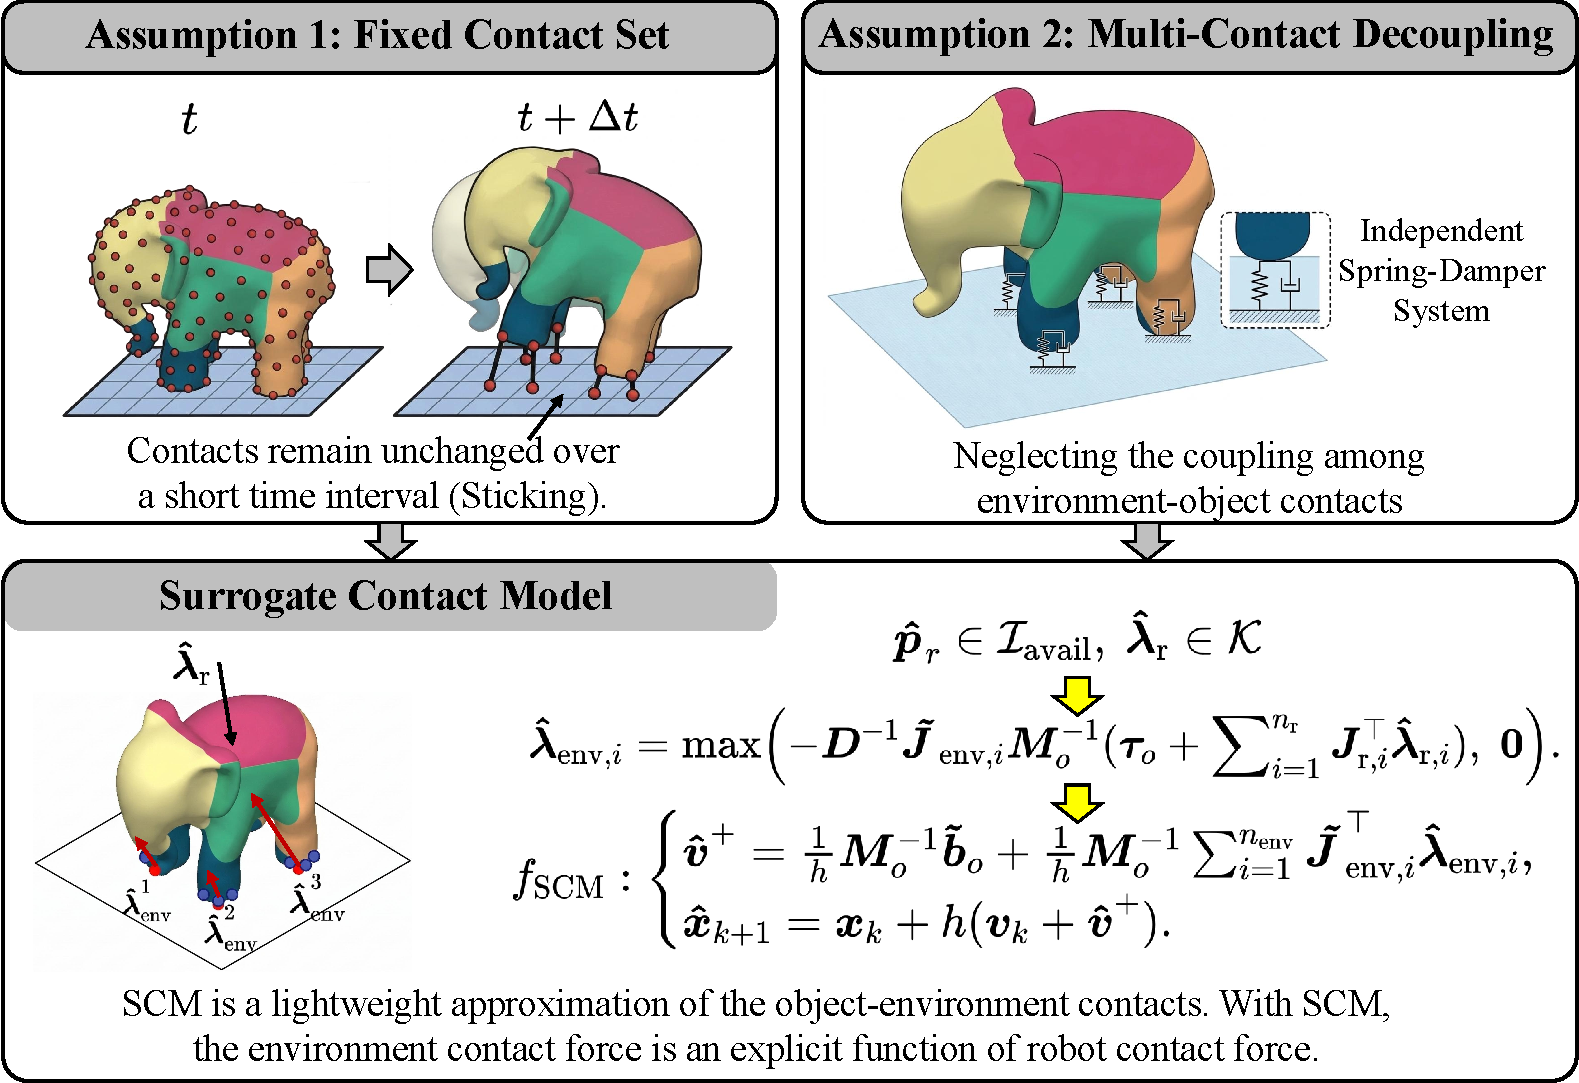
\includegraphics[width=\columnwidth]{figures/surrogate_contact_model.pdf}}
\caption{Illustration of SCM. SCM is a lightweight approximation of the object-environment contact, enabling fast contact selection optimization.}
\label{fig:stick1}
\end{figure}
\subsection{Formulation of CSO}\label{sec:cs_opt}

Integrating SCM into \eqref{equ:inner_loop}, we can obtain the formulation of CSO as: 
\begin{equation} 
\begin{aligned} 
\min_{\boldsymbol{\hat{p}}_{\text{r}} \in \mathcal{I}_{\text{avail}}}\min_{\boldsymbol{\hat{\lambda}}_{\text{r}} \in \mathcal{K}} & \quad 
\ell_{\text{cso}}\big(\boldsymbol{x}_{\textcolor{red}{T}}\big) \\ 
\text{s.t.} \quad
& \boldsymbol{\hat{\lambda}}_{\text{env}, i}
=
\max
\left(
-
\boldsymbol{D}^{-1}
\left(
\boldsymbol{\tilde{J}}_{\text{env},i} \boldsymbol{M}_o^{-1}\boldsymbol{\tilde{b}}_o
\boldsymbol{\tilde{\phi}}_{\text{env},i}
\right),
\;\boldsymbol{0}
\right), \\
& \boldsymbol{\hat{x}}_{k+1} 
= f_{\text{SCM}}(\boldsymbol{x}_k, \boldsymbol{\hat{p}}_{\text{r}}, \boldsymbol{\hat{\lambda}}_{\text{r}}), 
\quad k = 0, \dots, T-1, \\
& \textcolor{red}{|\hat{\lambda}_{r,i}^{t1}|\leq\mu_i\hat{\lambda}_{r,i}^{n}  , \ |\hat{\lambda}_{r,i}^{t2}|\leq\mu_i\hat{\lambda}_{r,i}^{n}}, \\
& 0 \le \hat{\lambda}^n_{r,i} \le \hat{\lambda}^n_{\text{max}}, \quad i = 0, \dots, n_{\text{r}}.
\end{aligned}\label{equ:csqp} 
\end{equation} 
By solving this discrete-continuous optimization problem, we can obtain the \rev{optimal contact location among candidate contact set $\boldsymbol{\hat{p}}_r^* \in \mathcal{I}_{\text{avail}}$} as guidance for the lower-level contact planning. Next, we discuss the details of CSO.
\subsubsection{Objective}
Despite the objective of CSO being to minimize the object pose cost as denoted in \eqref{equ:obj_pose_cost}, directly using $\ell_{\text{pose}}$ as the CSO objective $\ell_{\text{cso}}$ results in unstable contact strategies by blindly minimizing cost. In addition, the execution of the lower-level contact planning approach is inherently subject to delay, since the robot must physically approach and establish contact rather than instantaneously reaching the selected contact location. Therefore, the design of the CSO should explicitly consider the delay and avoid unstable behaviors that may cause frequent dynamic changes in the object pose. Therefore, we introduce the concept of an equivalence class of stable poses of an object as $\mathcal{X}_{\text{stab}}=\bigcup_{j=1}^{k}\mathcal{X}_{j}$,
where $\mathcal{X}_{j}$ denotes the $j$-th class of stable pose of the object and $\boldsymbol{x}_{\text{o}} \in \mathcal{X}_{j}$ is a statically stable pose at which the object can remain at rest on the table, with its center of mass projected within the support polygon. We define the transfer cost from the current object pose to the goal stable pose as:
\begin{equation}
\ell_{\text{stab}}(\boldsymbol{x}_o)
=
d(\boldsymbol{x}_o,\mathcal{X}_g),
\end{equation}
where $d(\cdot,\cdot)$ is a pose distance metric, $\mathcal{X}_j$ denotes the set of object poses associated with the $j$-th statically stable placement mode, and $\alpha>0$ is a weighting coefficient. We reformulate the CSO objective to prioritize reaching the goal pose set $\mathcal{X}_g$ from the current pose $\boldsymbol{x}_o$, and then minimize $\ell_{\text{pose}}$ in $\mathcal{X}_g$:
\begin{equation}\label{equ:objectice_obj}
\ell_{\text{cso}} =
\begin{cases}
\ell_{\text{stab}}, & \text{if } \boldsymbol{x}_o \notin \mathcal{X}_g, \\
\ell_{\text{pose}}, & \text{otherwise}.
\end{cases}
\end{equation}
The design of \eqref{equ:objectice_obj} effectively guides the gradient descent of CSO to select a more statically stable trajectory. Although this increases the control cost, it effectively prevents CSO from generating numerous unstable contact locations as priors, which would otherwise make the lower-level contact planning difficult to execute in practice.

 
\subsubsection{Solving CSO over Sampled Candidates}
The original contact dynamics in \eqref{equ:inner_loop} are non-differentiable because of the complementarity constraints and the non-smooth temporal evolution of the contact set, rendering the constraints non-differentiable. With the SCM, \eqref{equ:csqp} becomes a finite candidate search with a continuous force-optimization subproblem for each candidate. The SCM gradients can be computed via: 
\begin{equation} 
    \begin{aligned} 
    \frac{\partial \boldsymbol{x}_{k+1}}{\partial \boldsymbol{\lambda}_{\text{r},i}} 
&=
\frac{\partial \boldsymbol{x}_{k+1}}{\partial \boldsymbol{v}^{+}} 
\left( 
\frac{\partial \boldsymbol{v}^{+}}{\partial \boldsymbol{b}} 
\frac{\partial \boldsymbol{b}}{\partial \boldsymbol{\lambda}_r} 
+
\frac{\partial \boldsymbol{v}^{+}}{\partial \boldsymbol{\lambda}_{\text{env}}} 
\frac{\partial \boldsymbol{\lambda}_{\text{env}}}{\partial \boldsymbol{\lambda}_r} 
\right) \\ 
&=\boldsymbol{M}_o^{-1}\!\left(h\boldsymbol{J}_{\text{r},i}^\top  
+\frac{1}{h} \sum_{j=0}^{n_\text{env}}\boldsymbol{\tilde{J}}_{\text{env},j}^\top
\frac{\partial \boldsymbol{\lambda}_{\text{env},j}}{\partial \boldsymbol{\lambda}_{\text{r},i}}\right), 
\end{aligned} 
\end{equation} 
where the derivative $\frac{\partial \boldsymbol{\lambda}_{\text{env},j}}{\partial \boldsymbol{\lambda}_{\text{r},i}}$ is obtained by automatic differentiation on each fixed active set, or from the SoftPlus derivative at an activation boundary. The resulting map is piecewise smooth; with SoftPlus it is smooth everywhere. The objective function $\ell_{\text{cso}}$ is then differentiable for the continuous force subproblem, which is solved for each candidate using SNOPT, after which the candidate costs are enumerated.




\section{Contact Planning Optimization}\label{sec:cpo}

In this section, we introduce the CPO module for contact planning. CPO accepts the optimal contact location predicted by CSO as reference, and generates approaching and contact trajectories online. We will discuss the problem of designing a prior-guided contact planning. Then we design a ranking strategy as an expressive connection between contact planning and contact prior from contact selection module. Finally, we propose a novel objective formulation for prior-guided contact trajectory generation, and present two solvers for CPO.


\subsection{Problem Statement} 


Compared to CIMPC methods, CPO must additionally consider the guidance from the high-level module and generate the corresponding executable trajectory. Based on \eqref{eq:CIMPC_opt}, we define CPO as the single shooting problem:
\begin{equation}
    \begin{aligned}
\min_{\boldsymbol{u}_{0:N-1}} \quad & 
 {\textstyle \sum_{i=0}^{N-1}}  \ell_{\text{cpo}}(\boldsymbol{x}_k, \boldsymbol{u}_k, \boldsymbol{\hat{p}}^*_{\text{r}}) + V_f(\boldsymbol{x}_N) \\
\text{s.t.}\quad & \boldsymbol{x}_{k+1} = f(\boldsymbol{x}_k, \boldsymbol{u}_k), \quad k=0,\dots,\textcolor{red}{T}-1, \\
& \boldsymbol{x}_k \in \mathcal{X}, \quad k=0,\dots,\textcolor{red}{T}, \\
& \boldsymbol{u}_k \in \mathcal{U}, \quad k=0,\dots,\textcolor{red}{T}-1.
\end{aligned}\label{equ:origin_cpo_problem}
\end{equation}
Here $\boldsymbol{\hat{p}}^*_{\text{r}}$ is explicitly included in the objective function. We next investigate two key questions: in what form should contact prior guide contact planning, and how should a feasible approach and contact trajectory be defined mathematically?
\subsubsection{\textcolor{red}{Role of Contact Guidance}}
In the previous section, we discussed how CIMPC methods suffer from gradient sparsity and proposed CSO, which serves as a pointwise global search on the object and provide contact guidance. But this raises another open question: in what form should the guidance affect contact execution? The most straightforward approach is full coupling, where the contact planning strictly follows and executes the guidance from the CSO. \textcolor{red}{However, such a fully coupled scheme may compromise control robustness because the upper-level surrogate abstracts away detailed contact interactions. Moreover, the object-centric search performed by CSO does not explicitly account for robot morphology, resulting in an inherent gap between contact selection and execution. Moreover, contact-rich manipulation is inherently underdetermined, as numerous contact-wrench and contact-location trajectories can accomplish the same task. Strictly executing the CSO-optimal trajectory would therefore restrict this intrinsic solution diversity in robot–object interaction. To address this limitation, we introduce an objective-based contact planning module named CPO. Through the ranking strategy, the CPO balances the CSO-optimal contact against nearby and other candidate contacts, establishing a loose coupling between high-level contact selection and low-level contact planning. This design benefits from global-search guidance to escape local optima while preserving the flexibility of contact planning for robust execution.}





\subsubsection{\textcolor{red}{Contact Switching Trajectory}}\label{sec:feasible_contact_trajectory}

\textcolor{red}{Existing CIMPC methods mainly induce nearby contacts through attractive costs, without explicitly modeling the detouring motions required for either approaching designated contacts or switching between contacts. To incorporate the upper-level guidance, we define the approaching trajectory in the contact-free space $\mathcal{S}_{\mathrm{free}}$ as:}
\begin{itemize}
\item All intermediate waypoints lie in the collision-free space.
\item The terminal waypoint establishes contact, and the contact force lies within the friction cone.
\end{itemize}

As shown in Fig. \ref{fig:approaching_contact}, the robot--object interaction states form a low-dimensional manifold embedded in the full system state space. A detouring motion can be viewed as planning a kinodynamically feasible bridging manifold $\mathcal{S}_{\text{approach}}$ within the contact-free space $\mathcal{S}_{\text{free}}$, connecting two states on the contact manifold $\mathcal{S}_{\text{contact}}$. This is challenging for CIMPC methods because, as discussed above, $\mathcal{S}_{\text{free}}$ provides little informative contact-induced gradient for such transitions. To naturally bridge the approaching, contact, and contact-switching phases without relying on a discrete state machine, we formulate CPO under a unified objective that jointly governs contact execution and pre-contact detouring and approach motions.

\subsection{Ranking Strategy of Contact Locations}
\label{sec:cpo-ranking_strategy}

\textcolor{red}{
In addition to the optimal contact location $\boldsymbol{\hat{p}}^*_{\text{r}}$ from the CSO prediction, we always consider the nearest point $\boldsymbol{p}_{\text{near}}$ to the current robot configuration as a candidate contact location: 
\begin{equation}\label{equ:nearest}
\textcolor{red}{
\boldsymbol{p}_{\mathrm{near}}
=\arg\min_{\boldsymbol{p}_i\in\mathcal{I}_{\mathrm{avail}}}
\bigl\|\boldsymbol{p}_{\mathrm{ee}}
-\boldsymbol{p}^{\mathrm{ee}}_i\bigr\|_2,
}
\end{equation}
where $\boldsymbol{p}^{\mathrm{ee}}_i$ is the end-effector position
corresponding to contact at $\boldsymbol{p}_i$. We reformulate the problem \eqref{equ:origin_cpo_problem} as tracking the reference contact location $\boldsymbol{p}_{\text{ref}}$, where $\boldsymbol{p}_{\text{ref}}$ is generated in real time through a ranking strategy between $\boldsymbol{p}_{\text{near}}$ and $\boldsymbol{\hat{p}}^*_{\text{r}}$, i.e., $\boldsymbol{p}_{\text{ref}} \in \left \{ \boldsymbol{p}_{\text{near}}, \boldsymbol{\hat{p}}^*_{\text{r}} \right \} $. Accordingly, the ranking output determines whether to maintain the current contact or detach and switch to $\boldsymbol{\hat{p}}^*_{\mathrm{r}}$ in the contact phase, and whether to establish a nearby contact or detour toward $\boldsymbol{\hat{p}}^*_{\mathrm{r}}$ in the pre-contact phase. We next define the evaluation criteria for the ranking strategy. 
}

\textcolor{red}{
For each candidate contact location $\boldsymbol{p}_i$, the optimal cost reduction obtained from \eqref{equ:objectice_obj} is denoted as
$\Delta \ell_t^i
=\ell(\boldsymbol{x}_t)-\ell(\hat{\boldsymbol{x}}_t^+)$.
Based on the predicted cost reduction range of all candidate contact locations, $\left[\Delta\ell_t^{\mathrm{min}},\Delta\ell_t^{\mathrm{max}}\right]$, the relative ranking score of the nearby contact $\boldsymbol{p}_{\mathrm{near}}$ is defined as
}
\begin{equation}\label{equ:ranking1}
\textcolor{red}{
\rho_t=
\Pi_{[0,1]}\!\left(
\frac{
\Delta\ell_t^{\mathrm{near}}
-\Delta\ell_t^{\mathrm{min}}
}{\max(
\Delta\ell_t^{\mathrm{max}}
-\Delta\ell_t^{\mathrm{min}}, \epsilon)
}
\right),
}
\end{equation}
\textcolor{red}{
where the fraction performs min-max normalization and  $\Pi_{[0,1]}$ projects the resulting score onto $[0,1]$.
The ranking score $\rho_t$ indicates the relative improvement of the
nearby contact compared with all candidate contacts.
}

\textcolor{red}{
Next, we define a binary trigger variable $\kappa_t\in\{0,1\}$ to
determine whether the nearby contact is suitable for replacing the
CSO-selected contact:
}
\begin{equation}\label{equ:kappa}
\textcolor{red}{
\kappa_t=\mathbf{1}\!\left(\rho_t\geq\bar{\rho}\right),
}
\end{equation}
\textcolor{red}{
where $\bar{\rho}$ is a predefined ranking threshold and
$\mathbf{1}(\cdot)$ denotes the indicator function.
When $\kappa_t=1$, the nearby contact
$\boldsymbol{p}_{\mathrm{near}}$ provides a sufficiently competitive
cost reduction and can serve as a feasible reference contact.
Otherwise, the reference remains the CSO-selected contact
$\hat{\boldsymbol{p}}_{\mathrm r}^{*}$.
The trigger variable $\kappa_t$ therefore evaluates the feasibility of
the nearby contact and determines whether contact relocation is allowed.
}

\textcolor{red}{
To avoid frequent switching due to transient ranking variations, we apply a temporal hysteresis strategy to filter $\kappa_t$ when updating the reference contact.
}
\begin{equation}\label{equ:ranking}
\textcolor{red}{
\gamma_{t+1} =
\begin{cases}
0,
& \kappa_t=0,\quad t_{(\kappa=0)}\geq T_1,\\[2mm]
1,
& \kappa_t=1,\quad t_{(\kappa=1)}\geq T_2,\quad
t_{\mathrm{contact}}\geq T_3,\\[2mm]
\gamma_t,
& \mathrm{otherwise},
\end{cases}
}
\end{equation}
\textcolor{red}{
where $t_{(\kappa=0)}$ and $t_{(\kappa=1)}$ denote the consecutive
time counters for the two trigger conditions, and $t_{\mathrm{contact}}$
represents the duration of the current contact state.
The filtered trigger $\gamma_t$ is subsequently used in the CPO
objective formulation to determine whether the nearby contact or the
CSO-selected contact should be prioritized.
}

\textcolor{red}{
The overall ranking process repeatedly evaluates the nearby contact
under the current configuration. When $\gamma_t=1$, the nearby contact
$\boldsymbol{p}_{\mathrm{near}}$ is selected as the reference contact
$\boldsymbol{p}_{\mathrm{ref}}$; otherwise, the robot continues moving
toward the guidance
$\hat{\boldsymbol{p}}_{\mathrm r}^{*}$ generated by CSO.
The complete procedure is summarized in Algorithm~\ref{algo:ranking}. This hierarchical design establishes a weak coupling between CSO and CPO, allowing CPO to exploit the global search guidance from CSO while retaining the flexibility to autonomously determine feasible contact strategies.
}


\begin{algorithm}[t]
\caption{Ranking Strategy of CPO}
\label{algo:ranking}
\begin{algorithmic}[1]
\Require $\boldsymbol{\hat{p}}^*_r$ predicted by CSO, current robot configuration $\boldsymbol{q}_k$, threshold $\delta$
\Ensure Selected contact location $\boldsymbol{p}_{\text{ref}}$ and $\ell_{\text{lp}}$
\State Compute nearest point $\boldsymbol{p}_{\text{near}}$ to end-effector via \eqref{equ:nearest}
\State Evaluate contact cost $\ell_{\text{near}}$ via \eqref{equ:csqp}
\State Compute $\gamma$ via \eqref{equ:ranking1},  \eqref{equ:kappa}, \eqref{equ:ranking} \Comment{Ranking strategy}
\If{$\gamma =0$}
    \State $\boldsymbol{p}_{\text{ref}} = \boldsymbol{\hat{p}}^*_{\text{r}}$, $\ell_{\text{lp}}=\ell_{\text{lift}}$ \Comment{Lifting phase}
\Else
    \State $\boldsymbol{p}_{\text{ref}} \gets \boldsymbol{p}_{\text{near}}$, $\ell_{\text{lp}}=\ell_{\text{place}}$ \Comment{Placing phase}
\EndIf 
\end{algorithmic}
\end{algorithm}


\subsection{Formulation of CPO} 

Contact planning inherently consists of multiple phases, including approaching, contact establishment, and contact switching. However, the CIMPC formulation does not naturally support contact switching, because contact switching requires leaving $\mathcal{S}_{\text{contact}}$ and traversing the contact-free space $\mathcal{S}_{\text{free}}$, where the CIMPC objective provides no effective gradient information for trajectory optimization. To address this issue, we introduce a novel objective formulation that enables multi phases planning within a unified framework. The proposed formulation is general to different task settings and compatible with various optimization solvers.

As illustrated in Fig. \ref{fig:task_requirements}, the trajectory optimization is decomposed into three stages. First, the end-effector leaves the current contact and moves around the object toward an intermediate waypoint $\boldsymbol{p}_{\text{lift}}$ or pose $\boldsymbol{q}_{\text{lift}}$. This intermediate target guides the robot to reach a collision-free pre-contact configuration. Second, the end-effector is guided toward $\boldsymbol{p}_{\text{ref}}$ to establish contact. This design is inspired by footstep planning in legged robots \cite{acosta2025perceptive}. The corresponding cost formulations are introduced below.

\subsubsection{Lifting Phase} 

During the lifting phase, when the current nearest contact point $\boldsymbol{p}_{\text{near}}$ is infeasible, a hybrid potential field guides the robot to detach from the object and move above the guidance. It consists of a repulsive term from the object:
\begin{equation}
    \ell_{\text{obs}} = 
\begin{cases}
\textcolor{red}{-\log\left ( {\|\boldsymbol{p}_{\text{ee}} - \boldsymbol{p}_{\text{o}}\|^2 + \varepsilon} \right )} , & 
\text{if } \|\boldsymbol{p}_{\text{ee}} - \boldsymbol{p}_{\text{o}}\|^2 < \sigma, \\[8pt]
0, & \text{otherwise.}
\end{cases}
\end{equation}
and an attractive term toward the lifting point $\boldsymbol{p}_{\text{lift}}$ or lifting configuration $\boldsymbol{q}_{\text{lift}}$. The lifting target satisfies:
$\left \| \boldsymbol{p}_{\text{lift}}-\hat{\boldsymbol{p}}_r^* \right \|_2  = d $
or
$ \left \|\text{FK}({\boldsymbol{q}_{\text{lift}})}-\hat{\boldsymbol{p}}_r^*\right \|_2  = d$,
which guides the robot toward a position above $\hat{\boldsymbol{p}}_r^*$. The attractive potential is defined as:
\begin{equation}
    \textcolor{red}{\ell_{\text{att}} = \|\boldsymbol{p}_{\text{ee}} - \boldsymbol{p}_{\text{lift}}\|^2 }
    \quad \text{or} \quad 
    \ell_{\text{att}} = \|\boldsymbol{q}_{\text{ee}} - \boldsymbol{q}_{\text{lift}}\|^2.
\end{equation}
The lifting cost is formulated as:
\begin{equation}
    \ell_{\text{lift}} = w_{\text{att}} \, \ell_{\text{att}} + w_{\text{obs}} \, \ell_{\text{obs}}.
\end{equation}
This potential formulation explicitly encodes the lifting behavior and avoids optimization failure caused by gradient-sparse regions during contact breaking.

\subsubsection{Placing Phase}

During the placing phase, when the robot reaches a position above $\hat{\boldsymbol{p}}_r^*$, or when $\boldsymbol{p}_{\text{near}}$ is verified as a feasible contact location, the end-effector is guided to establish contact with the object. The placing phase is formulated by:
\begin{equation}
    \ell_{\text{place}} = w_{\text{con}}  \ell_{\text{con}} + w_{\text{o}} \ell_{\text{o}},
\end{equation}
where $\ell_{\text{con}}$ attracts the end-effector toward the reference contact point $\boldsymbol{p}_{\text{ref}}$, and $\ell_{\text{o}}$ attracts it toward the object center:
\begin{equation}
    \ell_{\text{con}} = \left\|\boldsymbol{p}_{\text{ee}} - \boldsymbol{p}_{\text{ref}}\right\|^2, 
    \quad 
    \ell_{\text{o}} = \left \| \boldsymbol{p}_{\text{o}} - \boldsymbol{p}_{\text{ee}} \right \|^2.
\end{equation}
Using only $\ell_{\text{con}}$ may fail to establish physical contact when the object mesh is inaccurate, since perception or projection errors can cause $\hat{\boldsymbol{p}}_r^*$ to deviate from the actual object surface. The additional term $\ell_{\text{o}}$ improves robustness against such errors.

\subsubsection{Switching Parameter}

The switching between lifting and placing behaviors is determined by the trigger $\gamma$ introduced in Section \ref{sec:cpo-ranking_strategy}. The overall lift-and-place cost is:
\begin{equation}
    \ell_{\text{lp}} = (1-\gamma)  \ell_{\text{lift}} + \gamma \ell_{\text{place}},
\end{equation}
where $\ell_{\text{lp}}$ is incorporated into the stage cost $\ell_{\text{cpo}}$ in \eqref{equ:origin_cpo_problem}. By defining the terminal cost $V_f$ identical to \eqref{equ:obj_pose_cost}, the CPO formulation is obtained as:
\begin{equation}\label{equ:cpo_formulation}
    \begin{aligned}
\min_{\boldsymbol{u}_k} \quad & 
 {\textstyle \sum_{i=0}^{N-1}}  \left (w_{\text{lp}} \ell_{\text{lp}}(\boldsymbol{x}_k, \boldsymbol{q}_k, \boldsymbol{u}_k, \boldsymbol{p}_{\text{ref}}) +w_{u}\left \| \boldsymbol{u}_{\textcolor{red}{k}} \right \|^2 \right ) +w_{\text{cso}}\ell_{\text{cso}} \\
\text{s.t.}\quad & \boldsymbol{x}_{\textcolor{red}{k+1}} = f_{\text{cf}}(\boldsymbol{x}_{\textcolor{red}{k}}, \boldsymbol{u}_{\textcolor{red}{k}}), \quad k=0,\dots,\textcolor{red}{T}-1, \\
& \boldsymbol{x}_k \in \mathcal{X}, \quad k=0,\dots,\textcolor{red}{T}, \\
& \boldsymbol{u}_k \in \mathcal{U}, \quad k=0,\dots,\textcolor{red}{T}-1.
\end{aligned}
\end{equation}

\begin{figure}[!t]
 \centerline{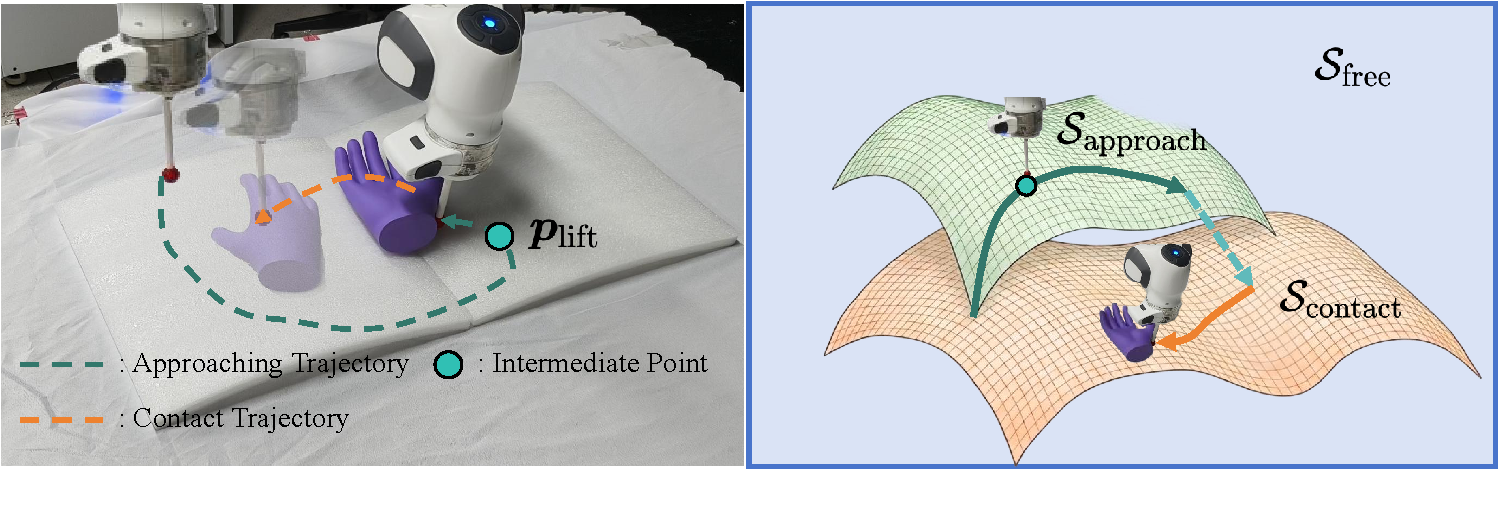
\includegraphics[width=\columnwidth]{figures/cpo_problem_def.pdf}}
\caption{(a) Illustrative example of a feasible approach and contact trajectory. (b) Explanation of CPO in a geometric perspective. CPO can be characterized as operating over two manifolds: contact states in $\mathcal{S}_{\text{contact}}$ and  approaching trajectories on the manifold $\mathcal{S}_{\text{approach}}$ embedded in the contact-free state space $\mathcal{S}_{\text{free}}$. CPO must not only generate contact trajectories on $\mathcal{S}_{\text{contact}}$ but also address the gradient-sparse issue and generate trajectories on $\mathcal{S}_{\text{approach}}$.}
\label{fig:approaching_contact}
\end{figure}

\begin{figure}[!t]
 \centerline{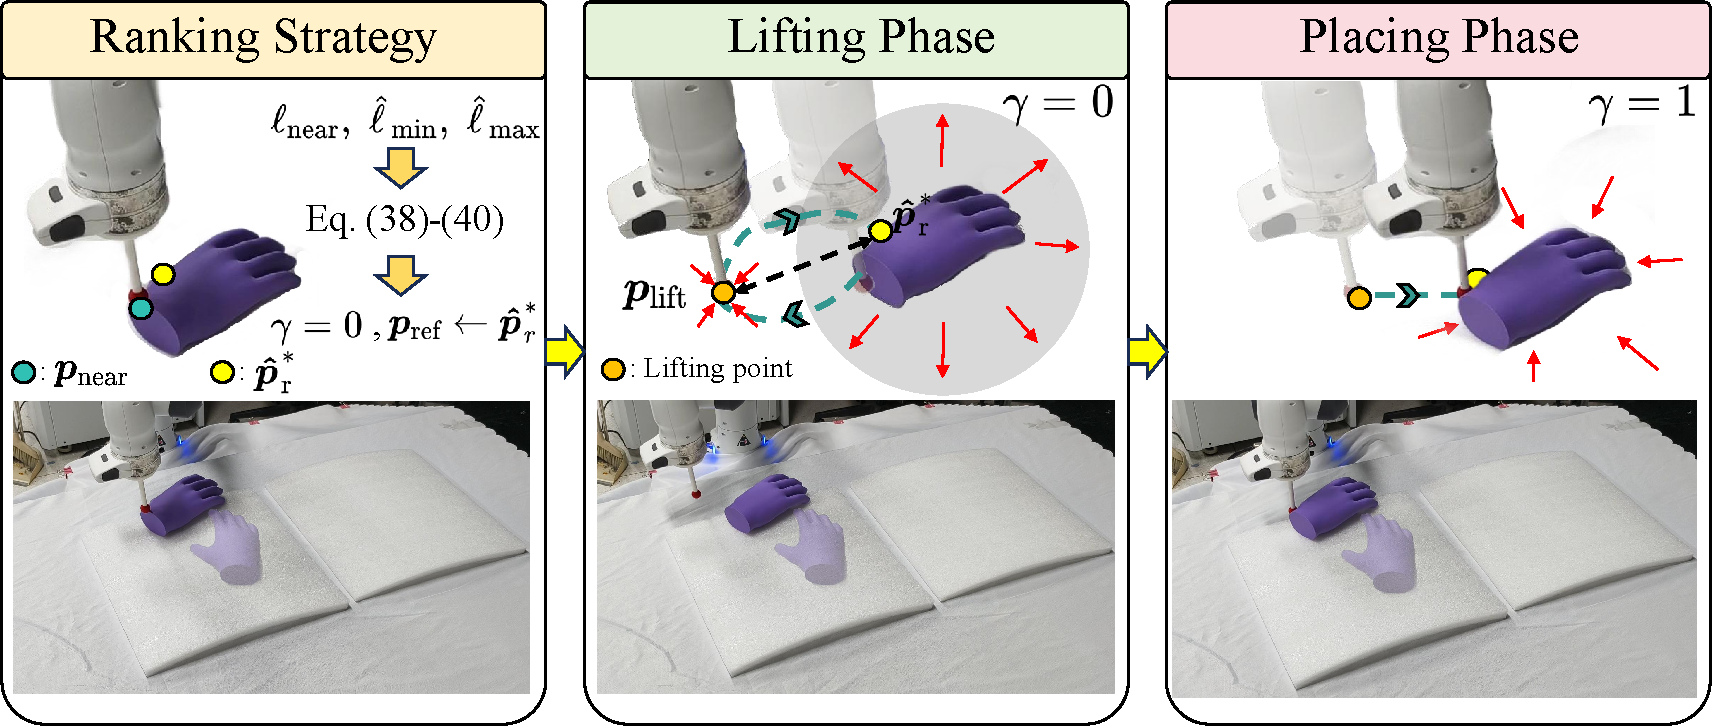
\includegraphics[width=\columnwidth]{figures/contact_planning_process.pdf}}
\caption{Illustration of the CPO-based contact planning module. (a) Ranking strategy. When $\boldsymbol{p}_{\text{near}}$ is evaluated infeasible, $\gamma$ turns to zero and $ \boldsymbol{p}_{\text{ref}} \gets \boldsymbol{\hat{p}}_r^*$. The evaluation runs continuously in real-time. (b) When $\gamma=0$,  the robot is guided by the potential field to $\boldsymbol{p}_{\text{lift}}$. (c) Once above $\hat{\boldsymbol{p}}_r^*$ or the nearest point $\boldsymbol{p}_{\text{ref}}$ to the robot is detected feasible via \eqref{equ:csqp}, $\gamma$ becomes 1 and an attractive potential is applied, guiding the robot to contact with the object.}
\label{fig:task_requirements}
\end{figure}

The formulation in \eqref{equ:cpo_formulation} preserves the favorable properties of the original CIMPC objective while enabling hybrid contact planning. Therefore, CPO can be interpreted as a prior-guided contact planning framework. We state the following lemma.

\begin{lemma}[Compatibility of $\ell_{\text{lp}}$ and $\ell_{\text{cso}}$]
$\ell_{\text{lp}}$ and $\ell_{\text{cso}}$ are non-conflicting objectives in CPO: minimizing the lift-and-place objective does not obstruct first-order improvement of the object manipulation objective.
\end{lemma}

\begin{proof}
    \renewcommand{\qedsymbol}{}
    See Appendix \ref{proof:lemma4}.
\end{proof}

\subsection{Solvers of CPO} 

Since CPO specifies the optimization formulation rather than a specific solver, various reactive motion planners can be adopted to generate contact trajectories. Below, we present two solvers employed in our experiments.


\subsubsection{Operational-Space Control}
\label{sec:osc_control}
We simplify the full-order contact planning problem to an end-effector point contact planning problem, avoiding high-DoF robot trajectory optimization. The resulting joint torques are generated by operational space control (OSC) \cite{nakanishi2008operational} to track the CPO output. Specifically, the state in \eqref{equ:cpo_formulation} is reduced to $\boldsymbol{s} \in \mathbb{R}^{10}$, consisting of the object position, object orientation represented by a quaternion, and the end-effector position $\boldsymbol{p}_{\text{ee}} \in \mathbb{R}^3$. Solving \eqref{equ:cpo_formulation} yields the control input $\boldsymbol{u} = \Delta \boldsymbol{p}_{\text{ee}}$.

Given the desired pose $(\boldsymbol{p}_d, \boldsymbol{R}_d)$ with $\boldsymbol{p}_d=\boldsymbol{p}_{\text{ee}}+\boldsymbol{u}$ and a preset $\boldsymbol{R}_d$, the position and orientation errors are computed as $\boldsymbol{e}_{\text{pos}} = \boldsymbol{u},
$ and $\boldsymbol{e}_{\text{R}} = \boldsymbol{R}_{\text{ee}}^\top \boldsymbol{R}_d$.
Converting $\boldsymbol{e}_{\text{R}}$ to quaternion form gives $\boldsymbol{e}_{\text{quat}} =
\begin{bmatrix}
\boldsymbol{\epsilon}_e, 
\eta_e
\end{bmatrix}^\top
\in \mathbb{R}^4$,
and after sign correction,
\begin{equation}
\boldsymbol{e}_{\text{quat}} \leftarrow
\begin{cases}
\boldsymbol{e}_{\text{quat}}, & \eta_e \ge 0,\\
-\boldsymbol{e}_{\text{quat}}, & \eta_e < 0,
\end{cases}
\qquad
\boldsymbol{e}_{\text{rot}} = -\boldsymbol{R}\boldsymbol{\epsilon}_e.
\end{equation}
By defining
$\boldsymbol{e}_{\text{pose}} =
\begin{bmatrix}
\boldsymbol{e}_{\text{pos}},
\boldsymbol{e}_{\text{rot}}
\end{bmatrix}^\top$,
the task-space and null-space torques are given by:
\begin{align}
\boldsymbol{\tau}_{\text{task}} &=
\boldsymbol{J}^{\top}(\boldsymbol{q})
\left(
-\boldsymbol{K}_x \boldsymbol{e}_{\text{pose}}
-\boldsymbol{D}_x \dot{\boldsymbol{x}}
\right), \\
\boldsymbol{\tau}_{\text{null}} &=
\left(
\boldsymbol{I} - \boldsymbol{J}^{\top}(\boldsymbol{J}^{\top})^{\dagger}
\right)
\left(
\boldsymbol{K}_{q}(\boldsymbol{q}_{\text{init}} - \boldsymbol{q})
- 2\sqrt{\boldsymbol{K}_{q}}\,\dot{\boldsymbol{q}}
\right),
\end{align}
and the final control torque is
$\boldsymbol{\tau} =
\boldsymbol{\tau}_{\text{task}}
+ \boldsymbol{\tau}_{\text{null}}
+ g(\boldsymbol{q})$. This controller is used in all simulations and real-world experiments in Section \ref{sec:experiment}, and is particularly suitable for tasks such as tabletop manipulation, where high orientation diversity is not critical.

\subsubsection{Sampling-based Motion Planner}

Another formulation is to directly solve the full-order planning problem of the robot. In this case, the state in \eqref{equ:cpo_formulation} is given by $\boldsymbol{x} \in \mathbb{R}^{7 + n_{\text{DoF}}}$, where $n_{\text{DoF}}$ denotes the number of robot DoFs. For this class of problems, we employ sampling-based MPC methods as the solver, such as MPPI \cite{williams2015model}. Recent studies  have demonstrated the impressive performance of MPPI in solving high-dimensional optimization problems for redundant robots, enabling real-time computation while avoiding issues related to gradient-based methods. The cost function is defined in the same manner as in the previous formulation, except that $\boldsymbol{p}_{\text{ee}}$ is computed via forward kinematics for the full-order problem. 
